\subsection{Tracking Multiple Points}

When tracking multiple points the same procedure as for one point is used.
Here only the image jacobians and $[du, dv]^T$ are stacked to $2 \cdot k \times 6$ and $2 \cdot k \times 1$ matrix, where $k$ is the number of points tracked.

The implemented algorithm takes in a vector of points of the marker that is wished tracked and a vector with the points in the image frame where these have to be tracked to.
A Dijkstra algorithm is then implemented to find the one-to-one mapping of marker points and their mapping in order to minimize the image displacement vector when tracking the marker.
%This algorithm hence performs best for small image displacements as the points tracked then are guaranteed to be mapped to the same point in the image coordinates.
This algorithm is guaranteed to map to the same point in the image coordinates for small displacements.
It is also possible to track all number of points in the image, given that there is at least the same number of points to map the marker to.
Since Dijkstra is used, the mapping with the least image displacements is always found.

The algorithm is however not suitable for large number of points.
%This is due to the exponential increase in number of ways to match $n$ found marker points to a corresponding or larger amount of points to map it to.
%In this project it was however decided not to use more than four points to track at a time and the algorithm is hence suitable for the given case.

%allows for a vector of points to be used when tracking multiple points.
%This is used to specify the set of locations in the image the different points are to be tracked to relative to the center of the image.

The visual servoing was tested using three points in the markers frame, namely (0,0,0), (0.1, 0, 0) and (0, 0.1, 0).
These were mapped to the image coordinates (0,0), (160,0) and (0, 160) in the image frame.
Figure \ref{fig:robotspeed_slow_3p}, \ref{fig:robotspeed_medium_3p} and \ref{fig:robotspeed_fast_3p} show the, as for the one point case, the robot velocity relative to the velocity limit.
The tool pose is plotted in figure \ref{fig:toolpose_3p_pos}, \ref{fig:toolpose_slow_3p_rpy}, \ref{fig:toolpose_medium_3p_rpy} and \ref{fig:toolpose_fast_3p_rpy}.
The translational part of the toll pose is only plotted along the z- and x-axis since the y values are constant.

The tracking error in pixels when following the marker is plotted in \ref{fig:trackingerror_slow_3p}, \ref{fig:trackingerror_medium_3p} and \ref{fig:trackingerror_fast_3p}.
All figures were plotted with a $\Delta t = 0.05$sec.



% ---------- Robot Velocity ----------
\begin{figure}[H]
\centering
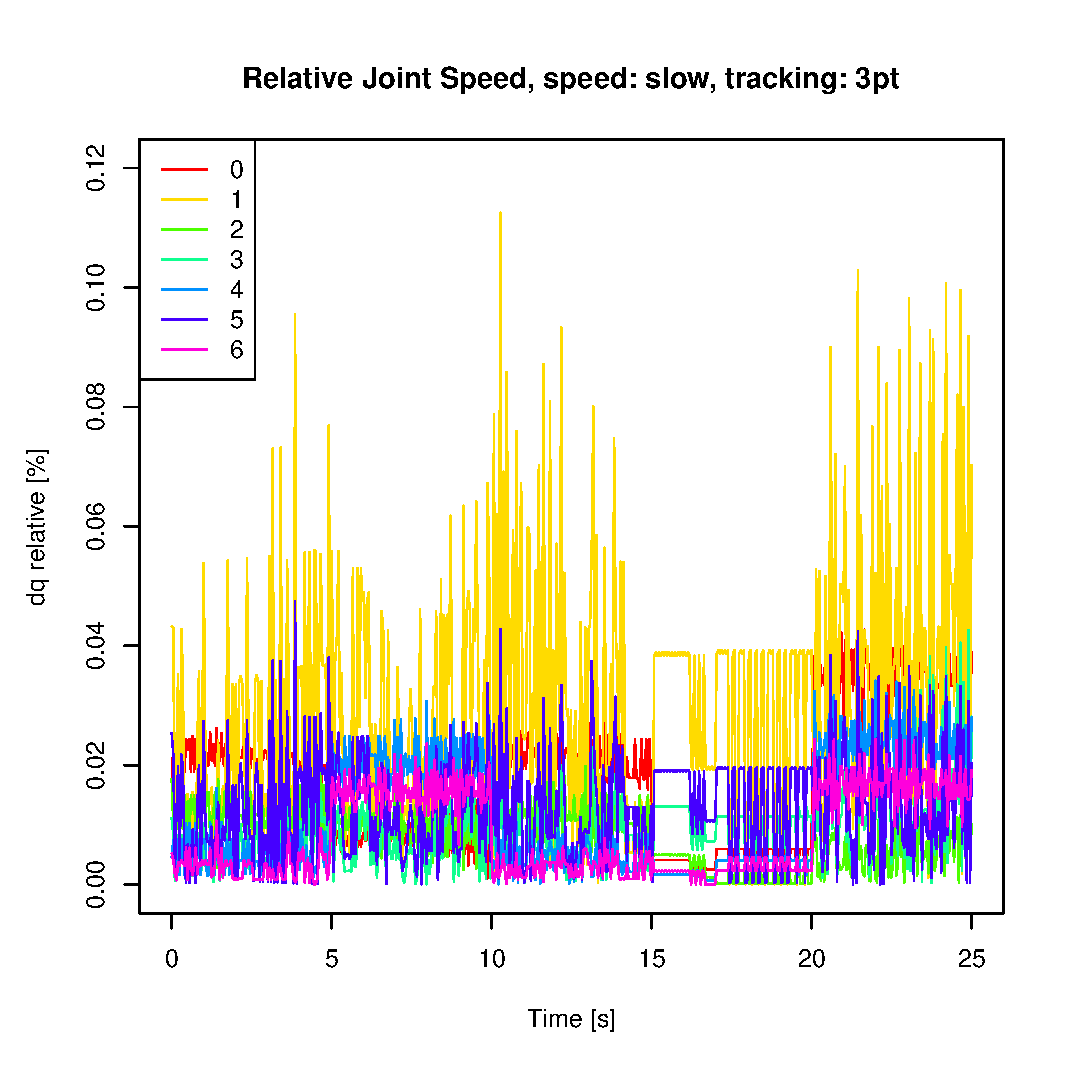
\includegraphics[width= \fullImageWidth]{graphics/robotics/relativeConfVel_slow_3pt}
\caption{Robot velocity relative to the velocity limit when tracking the slow marker movement.}
\label{fig:robotspeed_slow_3p}
\end{figure}

\begin{figure}[H]
\centering
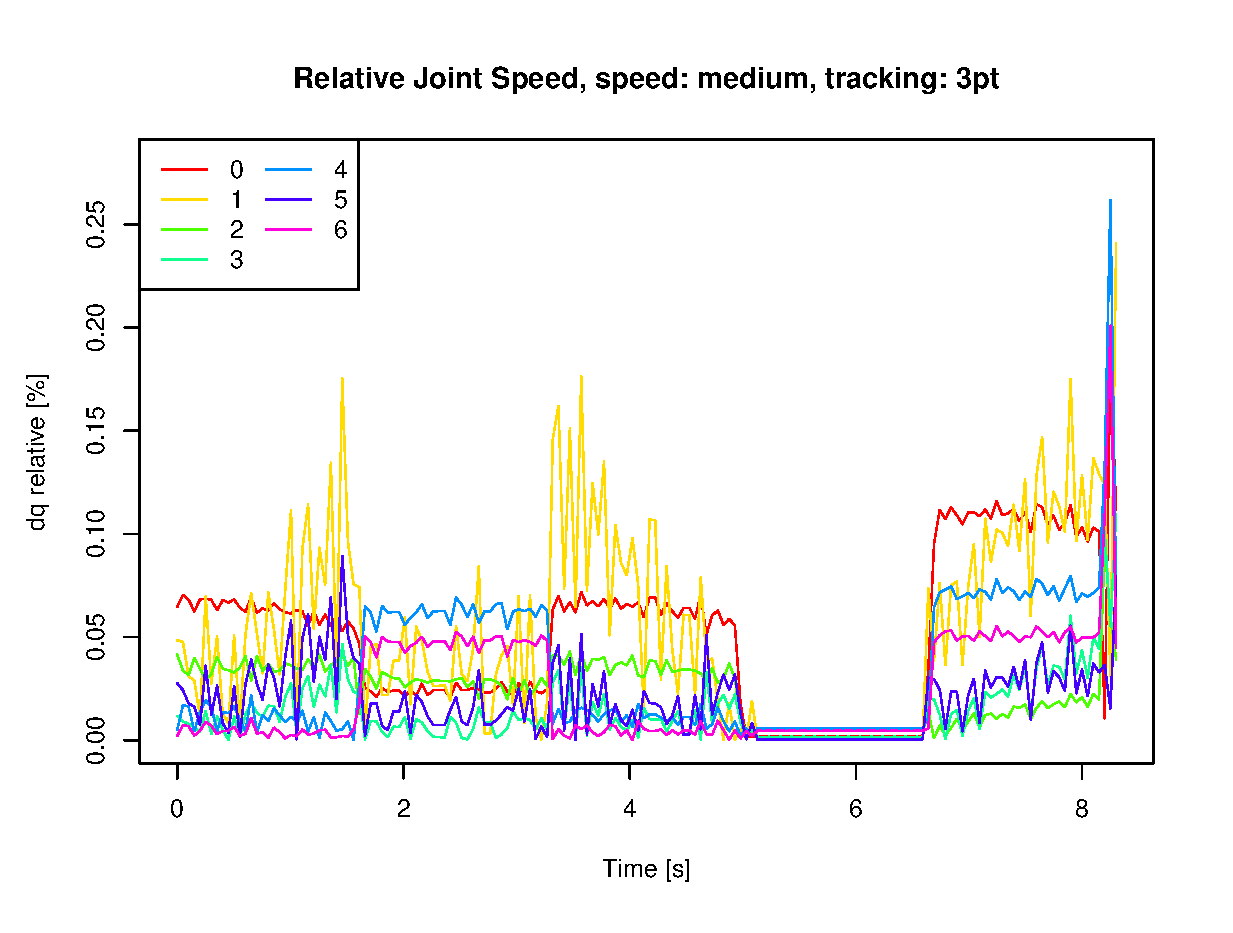
\includegraphics[width= \fullImageWidth]{graphics/robotics/relativeConfVel_medium_3pt}
\caption{Robot velocity relative to the velocity limit when tracking the medium marker movement.}
\label{fig:robotspeed_medium_3p}
\end{figure}

\begin{figure}[H]
\centering
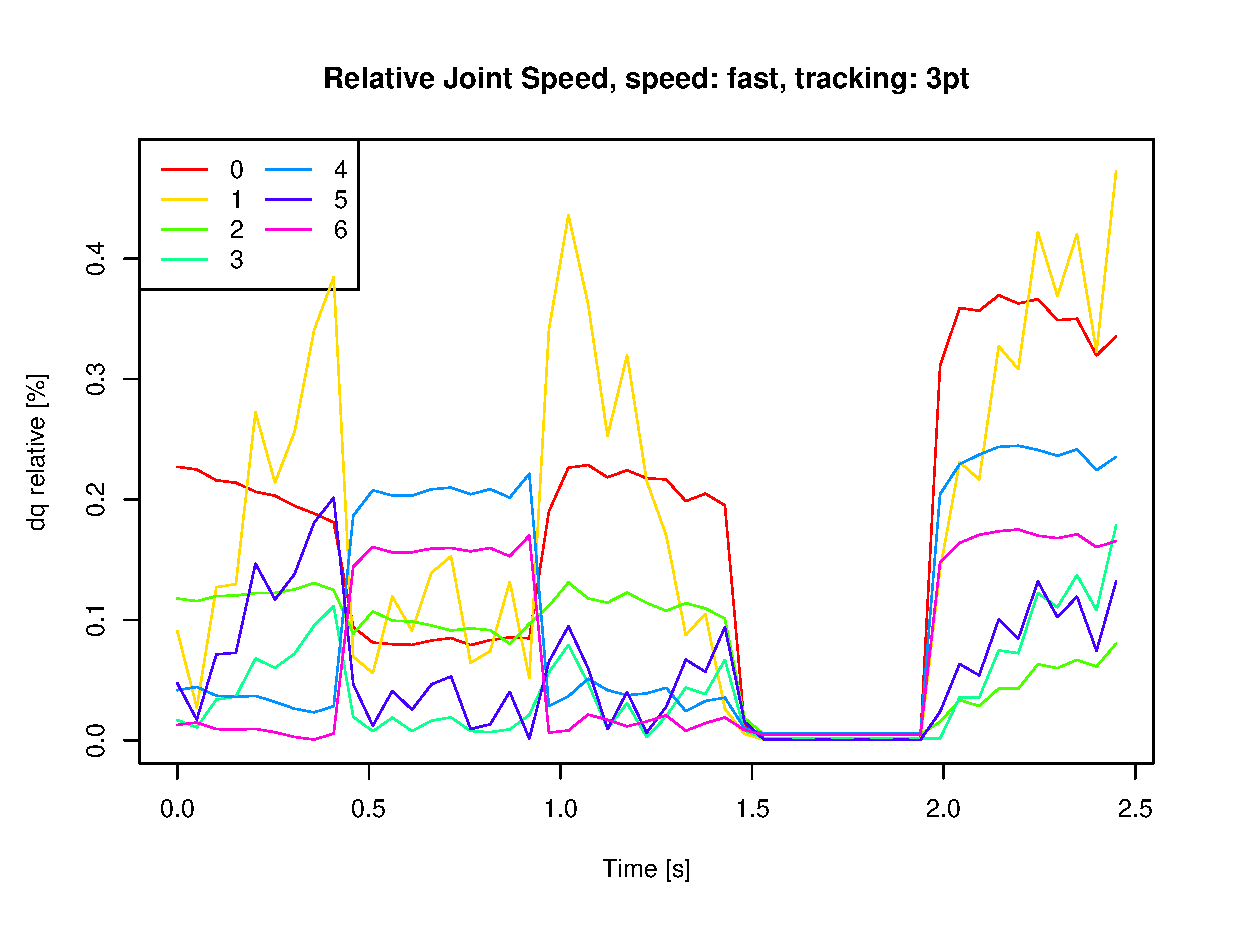
\includegraphics[width= \fullImageWidth]{graphics/robotics/relativeConfVel_fast_3pt}
\caption{Robot velocity relative to the velocity limit when tracking the fast marker movement.}
\label{fig:robotspeed_fast_3p}
\end{figure}


% ---------- Tool Pose ----------
\begin{figure}[H]
\centering
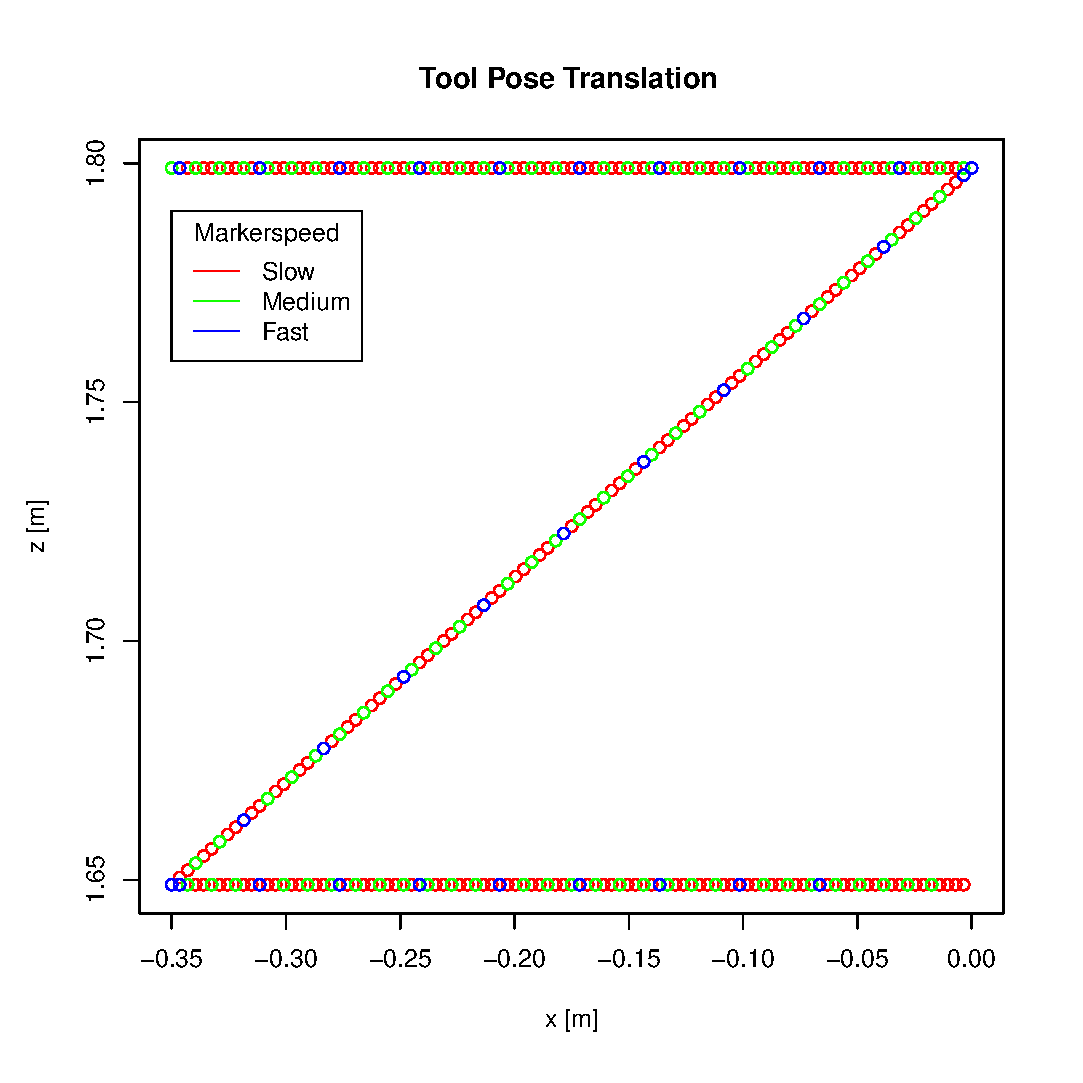
\includegraphics[width= \fullImageWidth]{graphics/robotics/toolPose_3pt_pos}
\caption{Translational part of tool pose when tracking three points.}
\label{fig:toolpose_3p_pos}
\end{figure}


\begin{figure}[H]
\centering
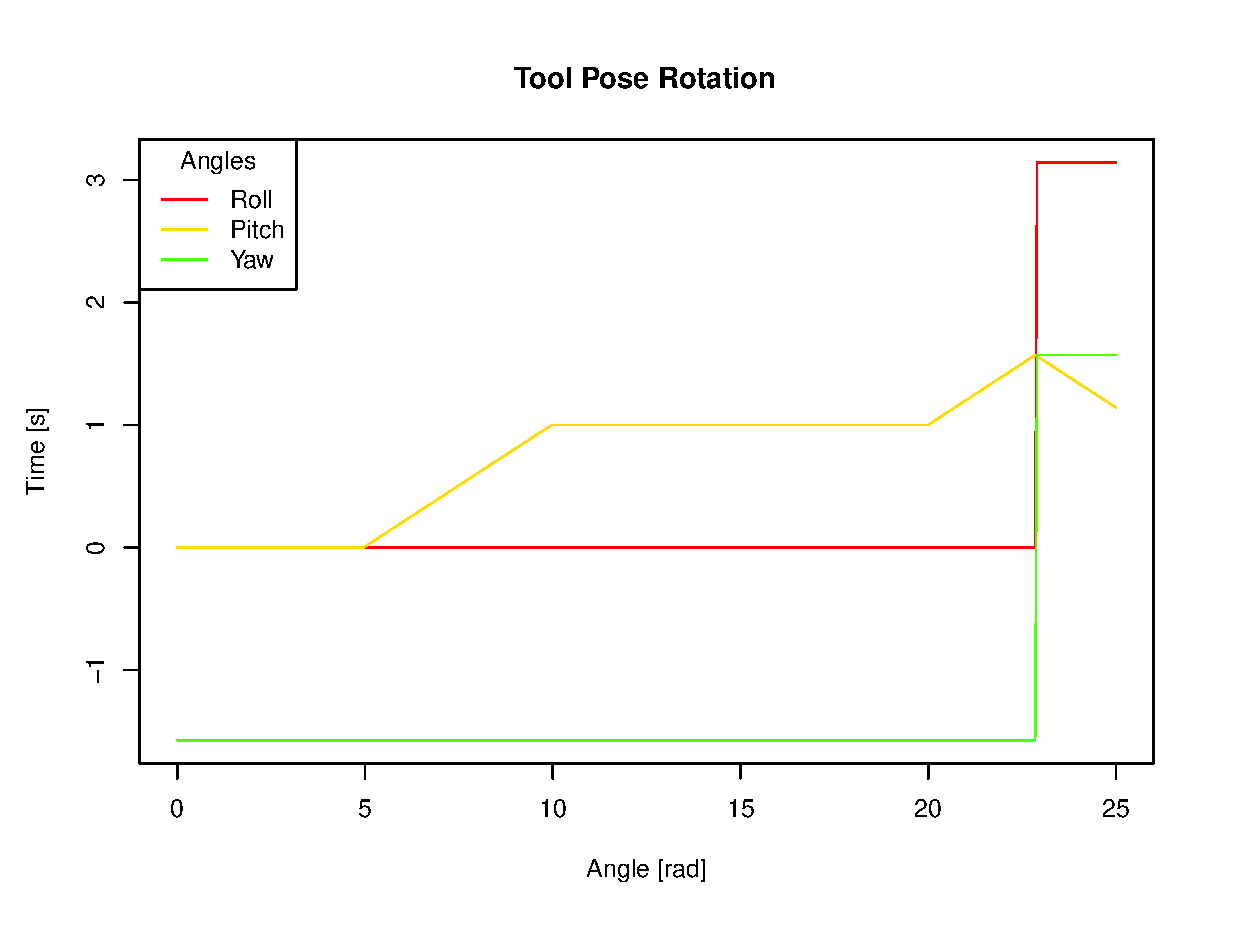
\includegraphics[width= \fullImageWidth]{graphics/robotics/toolPose_slow_3pt}
\caption{RPY part of tool pose. Using the slow marker movement while tracking 3 point.}
\label{fig:toolpose_slow_3p_rpy}
\end{figure}

\begin{figure}[H]
\centering
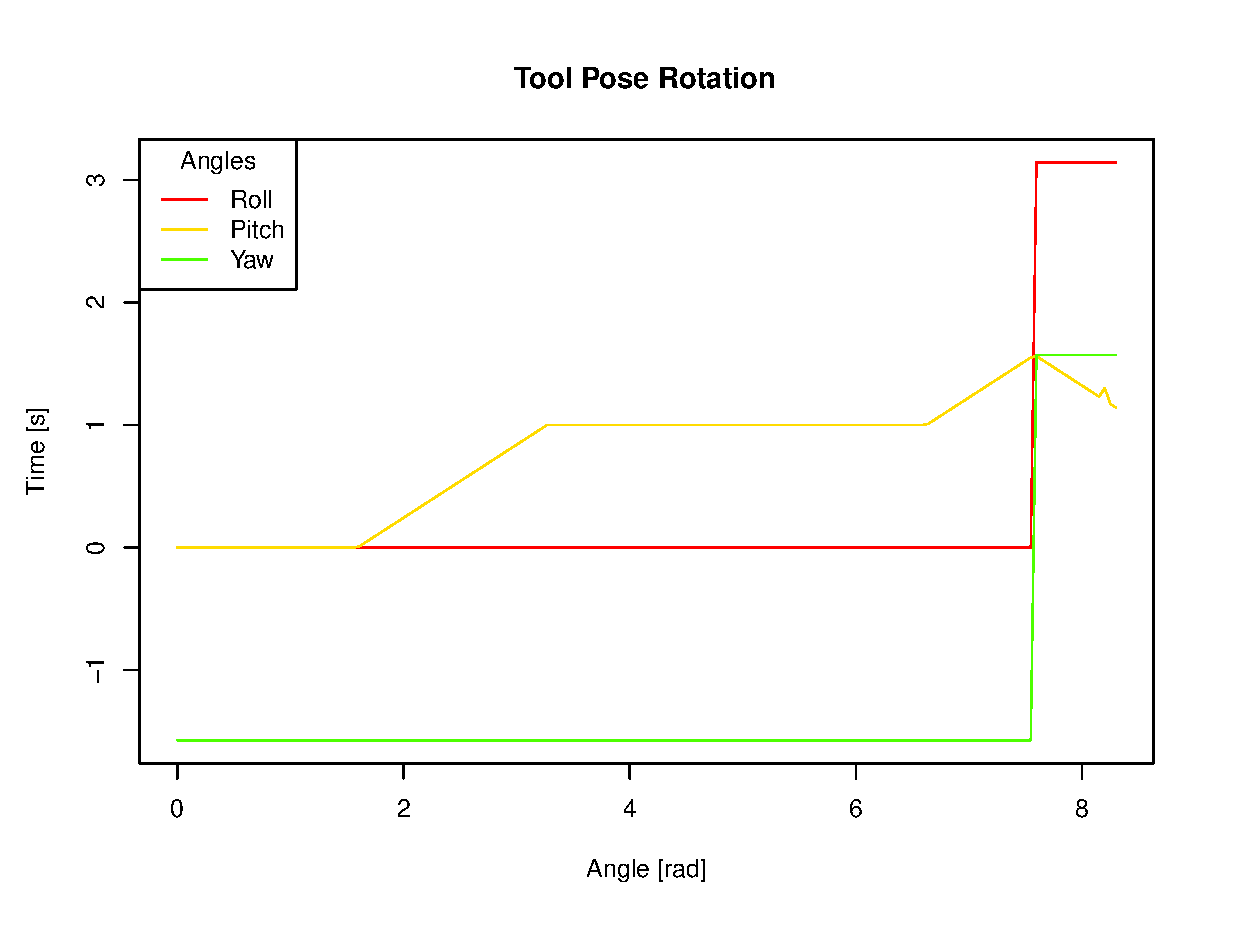
\includegraphics[width= \fullImageWidth]{graphics/robotics/toolPose_medium_3pt}
\caption{RPY part of tool pose. Using the medium marker movement while tracking 3 point.}
\label{fig:toolpose_medium_3p_rpy}
\end{figure}

\begin{figure}[H]
\centering
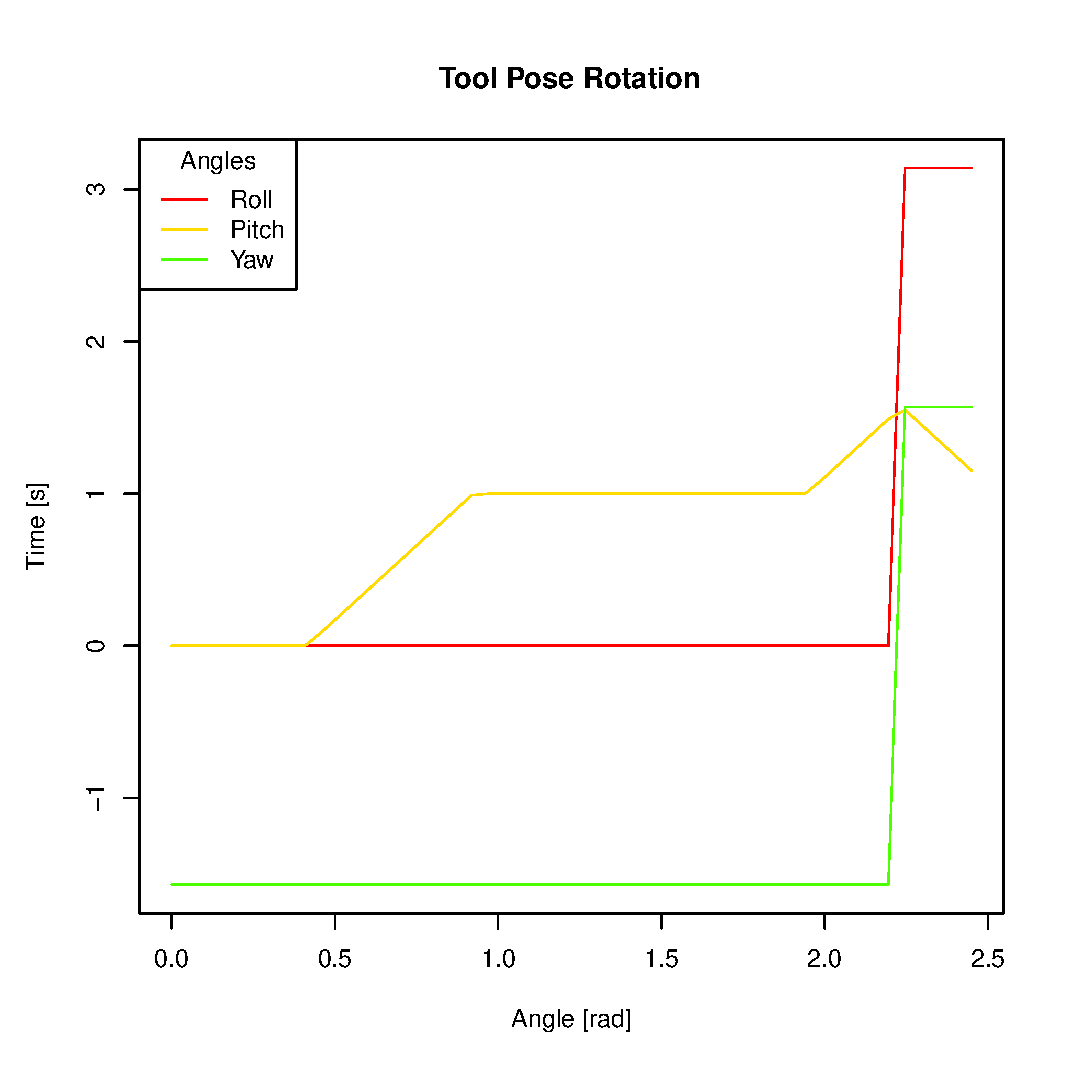
\includegraphics[width= \fullImageWidth]{graphics/robotics/toolPose_fast_3pt}
\caption{RPY part of tool pose. Using the fast marker movement while tracking 3 point.}
\label{fig:toolpose_fast_3p_rpy}
\end{figure}


% ---------- Tracking Error ----------
\begin{figure}[H]
\centering
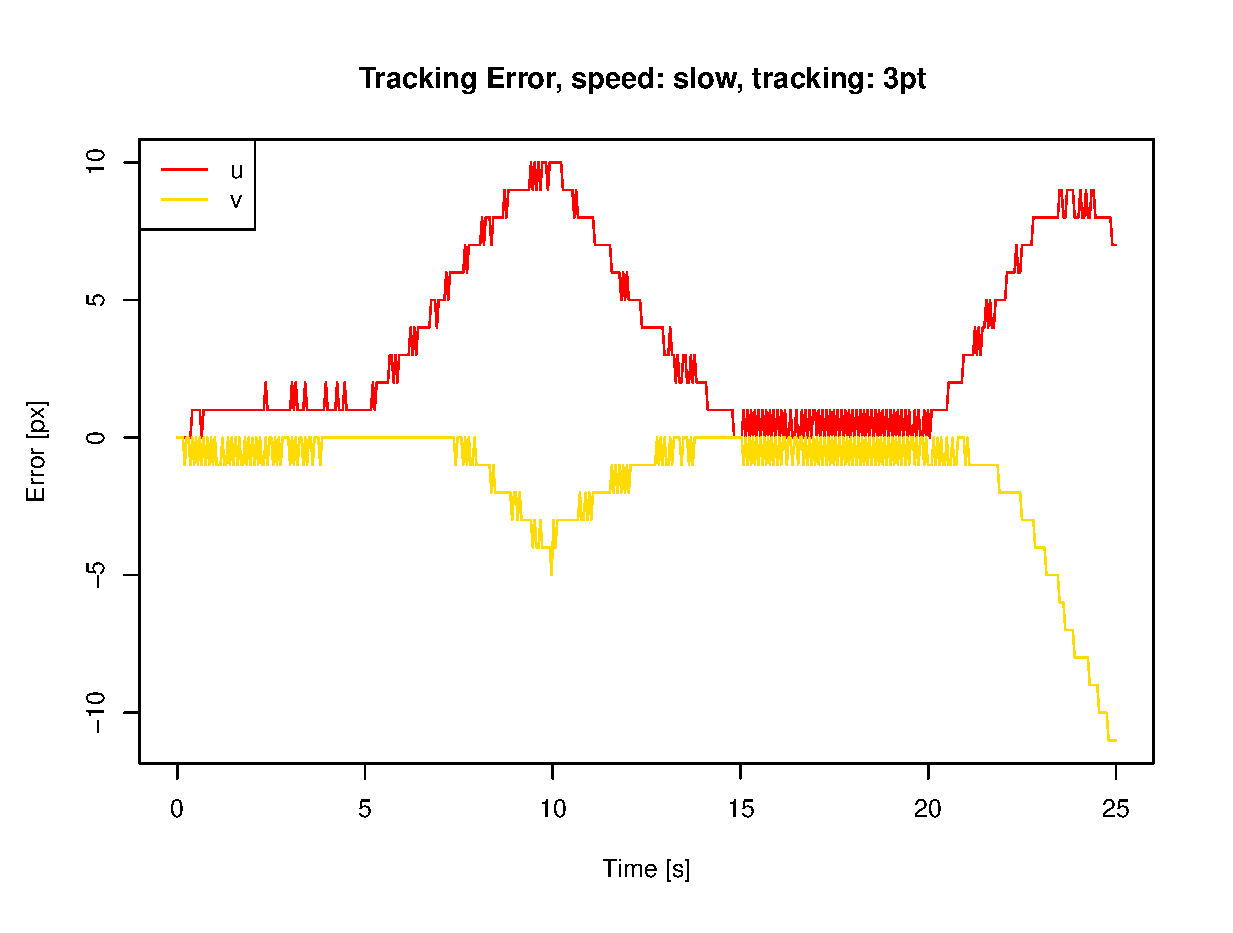
\includegraphics[width= \fullImageWidth]{graphics/robotics/trackingError_slow_3pt}
\caption{Tracking error in euclidean distance [px].
Following the marker for the slow marker movement.}
\label{fig:trackingerror_slow_3p}
\end{figure}

\begin{figure}[H]
\centering
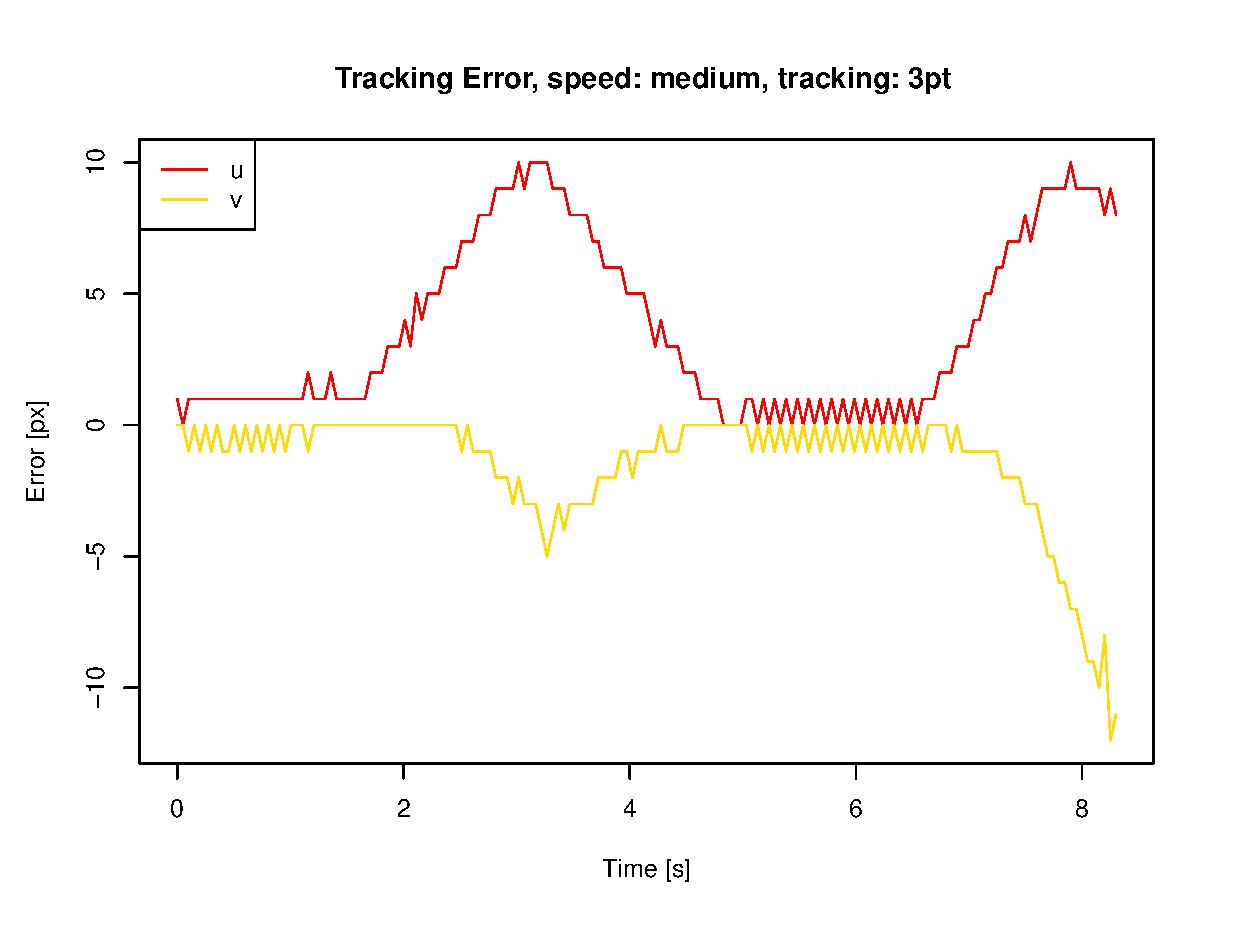
\includegraphics[width= \fullImageWidth]{graphics/robotics/trackingError_medium_3pt}
\caption{Tracking error in euclidean distance [px].
Following the marker for the medium marker movement.}
\label{fig:trackingerror_medium_3p}
\end{figure}

\begin{figure}[H]
\centering
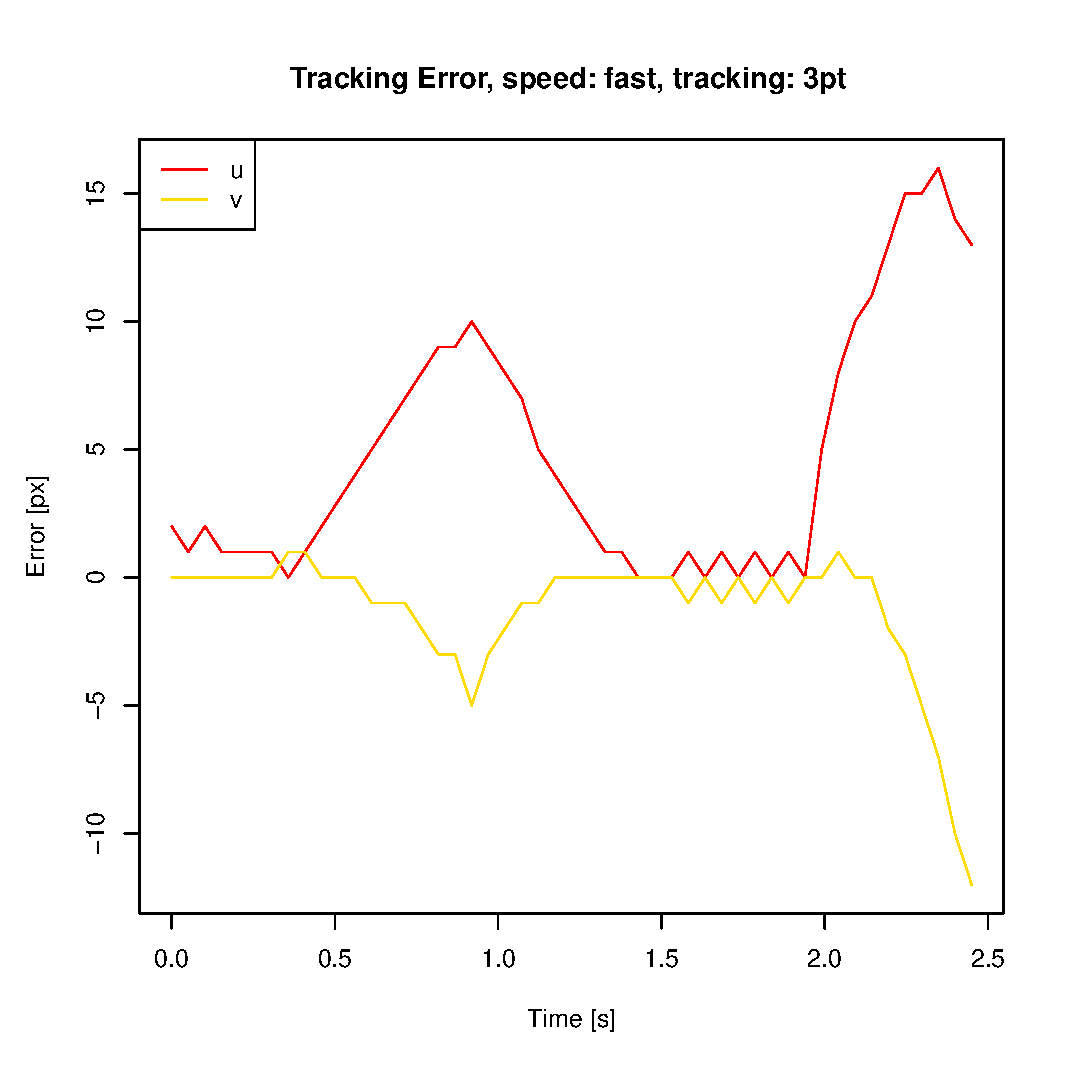
\includegraphics[width= \fullImageWidth]{graphics/robotics/trackingError_fast_3pt}
\caption{Tracking error in euclidean distance [px].
Following the marker for the fast marker movement.}
\label{fig:trackingerror_fast_3p}
\end{figure}

%As can be seen on the plots of the tool pose, then these are more or less identical.
It was found that in none of the cases was the velocity constraint violated for all of the datasets down to a $\Delta t = 0.05$ seconds in between each frame.
The tracking error does also increase as the marker movement speed increases, but the path taken by the robot tool is more or less the same for all of the datasets in the positional part as when tracking one point.
The velocity the robot is moving with is, however, higher than for one point since the robot is rotating with the marker.
